\section{Klasse Design}
\label{sec:klasse_design}
Som beskrevet i \cref{sec:klasse_teori} er det vigtig at få lave en model der modelere de ting fra virkeligheder som programmet skal arbejde med. Denne sektion vil dokumenter de grundlæggende modeller, som programmet er bygget op efter. 

For at give et overblik over klassehierarkiet er der lavet et UML-klassediagram som ses på \cref{fig:UML}. På diagrammet kan man se de vigtigste klasser der er brugt i løsningen. Af diagrammet fremgår også klassernes relationer.

De følgende under sektion beskriver programmets primære klasser og hvilken data som er inderholdt i klasserne.

\begin{figure}
  \label{fig:UML}  
  \centering
  \vspace*{-4.5cm}
  \thispagestyle{empty}
  \makebox[\textwidth]{
    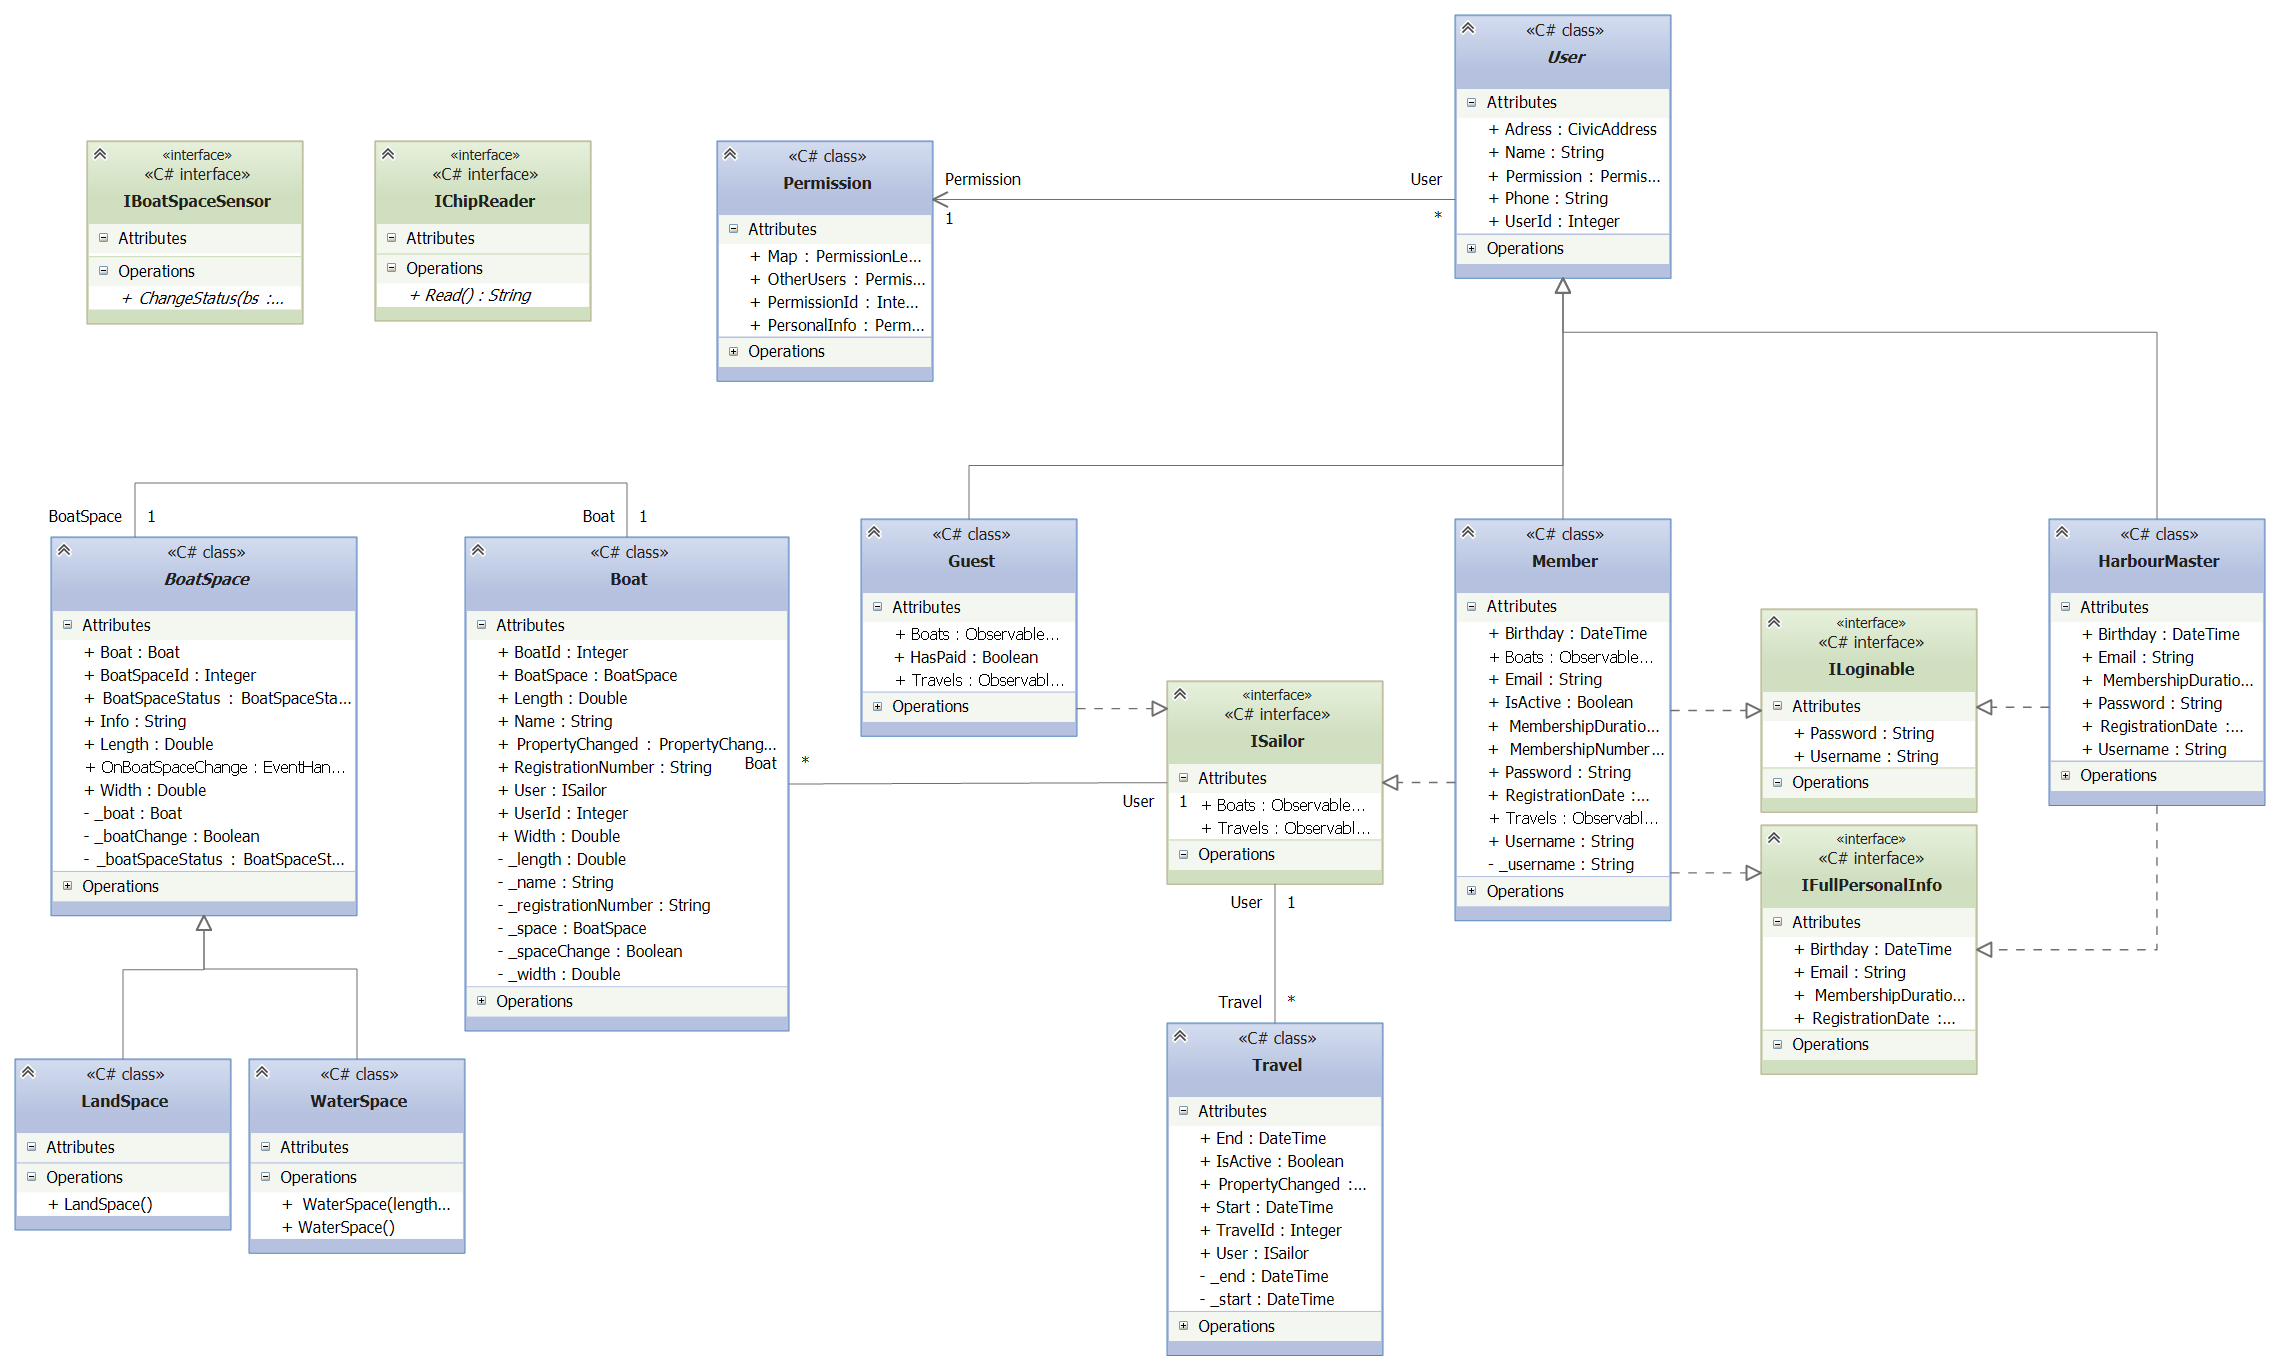
\includegraphics[width=1.2\paperwidth, angle = 270]{UML.png}
  }
 	\caption{UML-klassediagram over klasser der bruges til at modellere løsningen.}
 	\label{fig:UML}
\end{figure}

\subsection{Modellering af Brugere}
\label{sub:brugere_af_programmet}

I klassehierarkiets top ligger den abstrakte klasse \enquote{User}. En \enquote{User} er en generel bruger af systemet. Denne klasse definerer alle fællestræk de nedvarende klasser skal have. Dette inkluderer brugerrettigheder og basale informationer som telefonnummer, navn og adresse. Der findes tre forskellige interfaces, der indeholder forskellige informationer om brugere: \enquote{IFullPersonalInfo}, \enquote{ISailor}, \enquote{ILoginable}.

Subklasserne til \enquote{User} opdeler brugere som enten medlemmer af klubben, gæster eller havnefoged. Til disse tre brugertyper bruges klasserne \enquote{HarbourMaster}, \enquote{Guest} og \enquote{Member}. Denne opdeling er lavet fordi der indgår forskellige felter på tværs af disse subklasser. 

\sinote{Definer mere præcist opdelingen}

For at differentiere subklasserne, implementeres forskellige kombinationer af interfaces. Eksempelvis må en havnefoged ikke have en båd, og derfor implementerer klassen \enquote{HarbourMaster} ikke \enquote{ISailer} interfacet. Til gengæld deler \enquote{HarbourMaster}, \enquote{IFullPersonalInfo} og \enquote{ILoginable} med \enquote{Member} klassen, da de begge har behov for at gemme mere personinformation, samt at kunne logge ind med brugernavn/medlemsnummer.

\subsection{Modellering af Rejser}
\label{sub:rejser}

En medlems rejse modelleres med klassen \enquote{Travel}. Den indeholder information om rejsen start- og slutdato. \enquote{Travels} bruges også til at angive hvor lang tid en gæst ligger i havnen. \enquote{Travel} implementere \enquote{IEquatable} interfacet, som gør det muligt at sammenligne med andre klasser af samme type. Klasser der implementere ISailor indeholder en liste af \enquote{Travels}.

\subsection{Modellering af Både}
\label{sub:bade}

Der er lavet en klasse til både, der hedder \enquote{Boat}. Denne klasse bruges til at gemme data tilhørende en båd. Der gemmes dens navn og størrelse, så man kan tjekke hvorvidt en given plads er stor nok til at rumme båden.

Der er to klasser til repræsentation af bådpladser. Klassen \enquote{WaterSpace} modellere vandpladser og \enquote{LandSpace} modellere landplads. Begge disse klasser nedarver fra klassen \enquote{BoatSpace}, som indeholder generelle informationer om bådpladser.

\sinote{Flere klasser skal beskrives}
